\section{\textbf{Manufacturing}}\label{sec:4}
    For this project two PCB were made, hence in the presentation will be used two motors.
    As the simulation (see Section~\ref{sec:3}) proved that the designed circuit works as intended the physical components were assembled in a breadboard for further testing and validation before the final manufacturing \todo{complete with relevant information about final board}. Figure~\ref{fig:proto_h} shows the circuit properly assembled. This circuit's evaluation will be further discussed in Section~\ref{sec:5}.

    \subsubsection{Fritizing} % (fold)
    \label{ssub:fritizing}
        For aid the design of the printed circuit board it was used the software Fritizing\footnote{\url{http://fritzing.org/home/}}, that is an open source software used worldwide by hobbyists and it is an Electronic Design Automation software
        The Fritizing has 3 environments, shown in Figure~\ref{fig:breadboard}, they are breadboard, schematic and PCB, it was used only the schematic and design environments since the breadboard already has been evaluated.
    \todo{Show the fritzing environment, the schematics, board design and board manufacturing}
    % subsubsection fritizing (end)

    \subsubsection{Design} % (fold)
    \label{ssub:printing}

    % subsubsection printing (end)

    \subsubsection{Printing} % (fold)
    \label{ssub:printing}
    
    % subsubsection printing (end)
	\todo{TALK ABOUT CIRCUIT PRINTING}
	
	
	For the sake of validation the Magician Chasis \todo{picture and ref} was properly assembled and each board produced was attached to a motor which was connected to a wheel of the Chasis. This allowed the vehicle to move forward or backward depending on the switch's position.
\begin{figure}[t]
\centering
\centering%
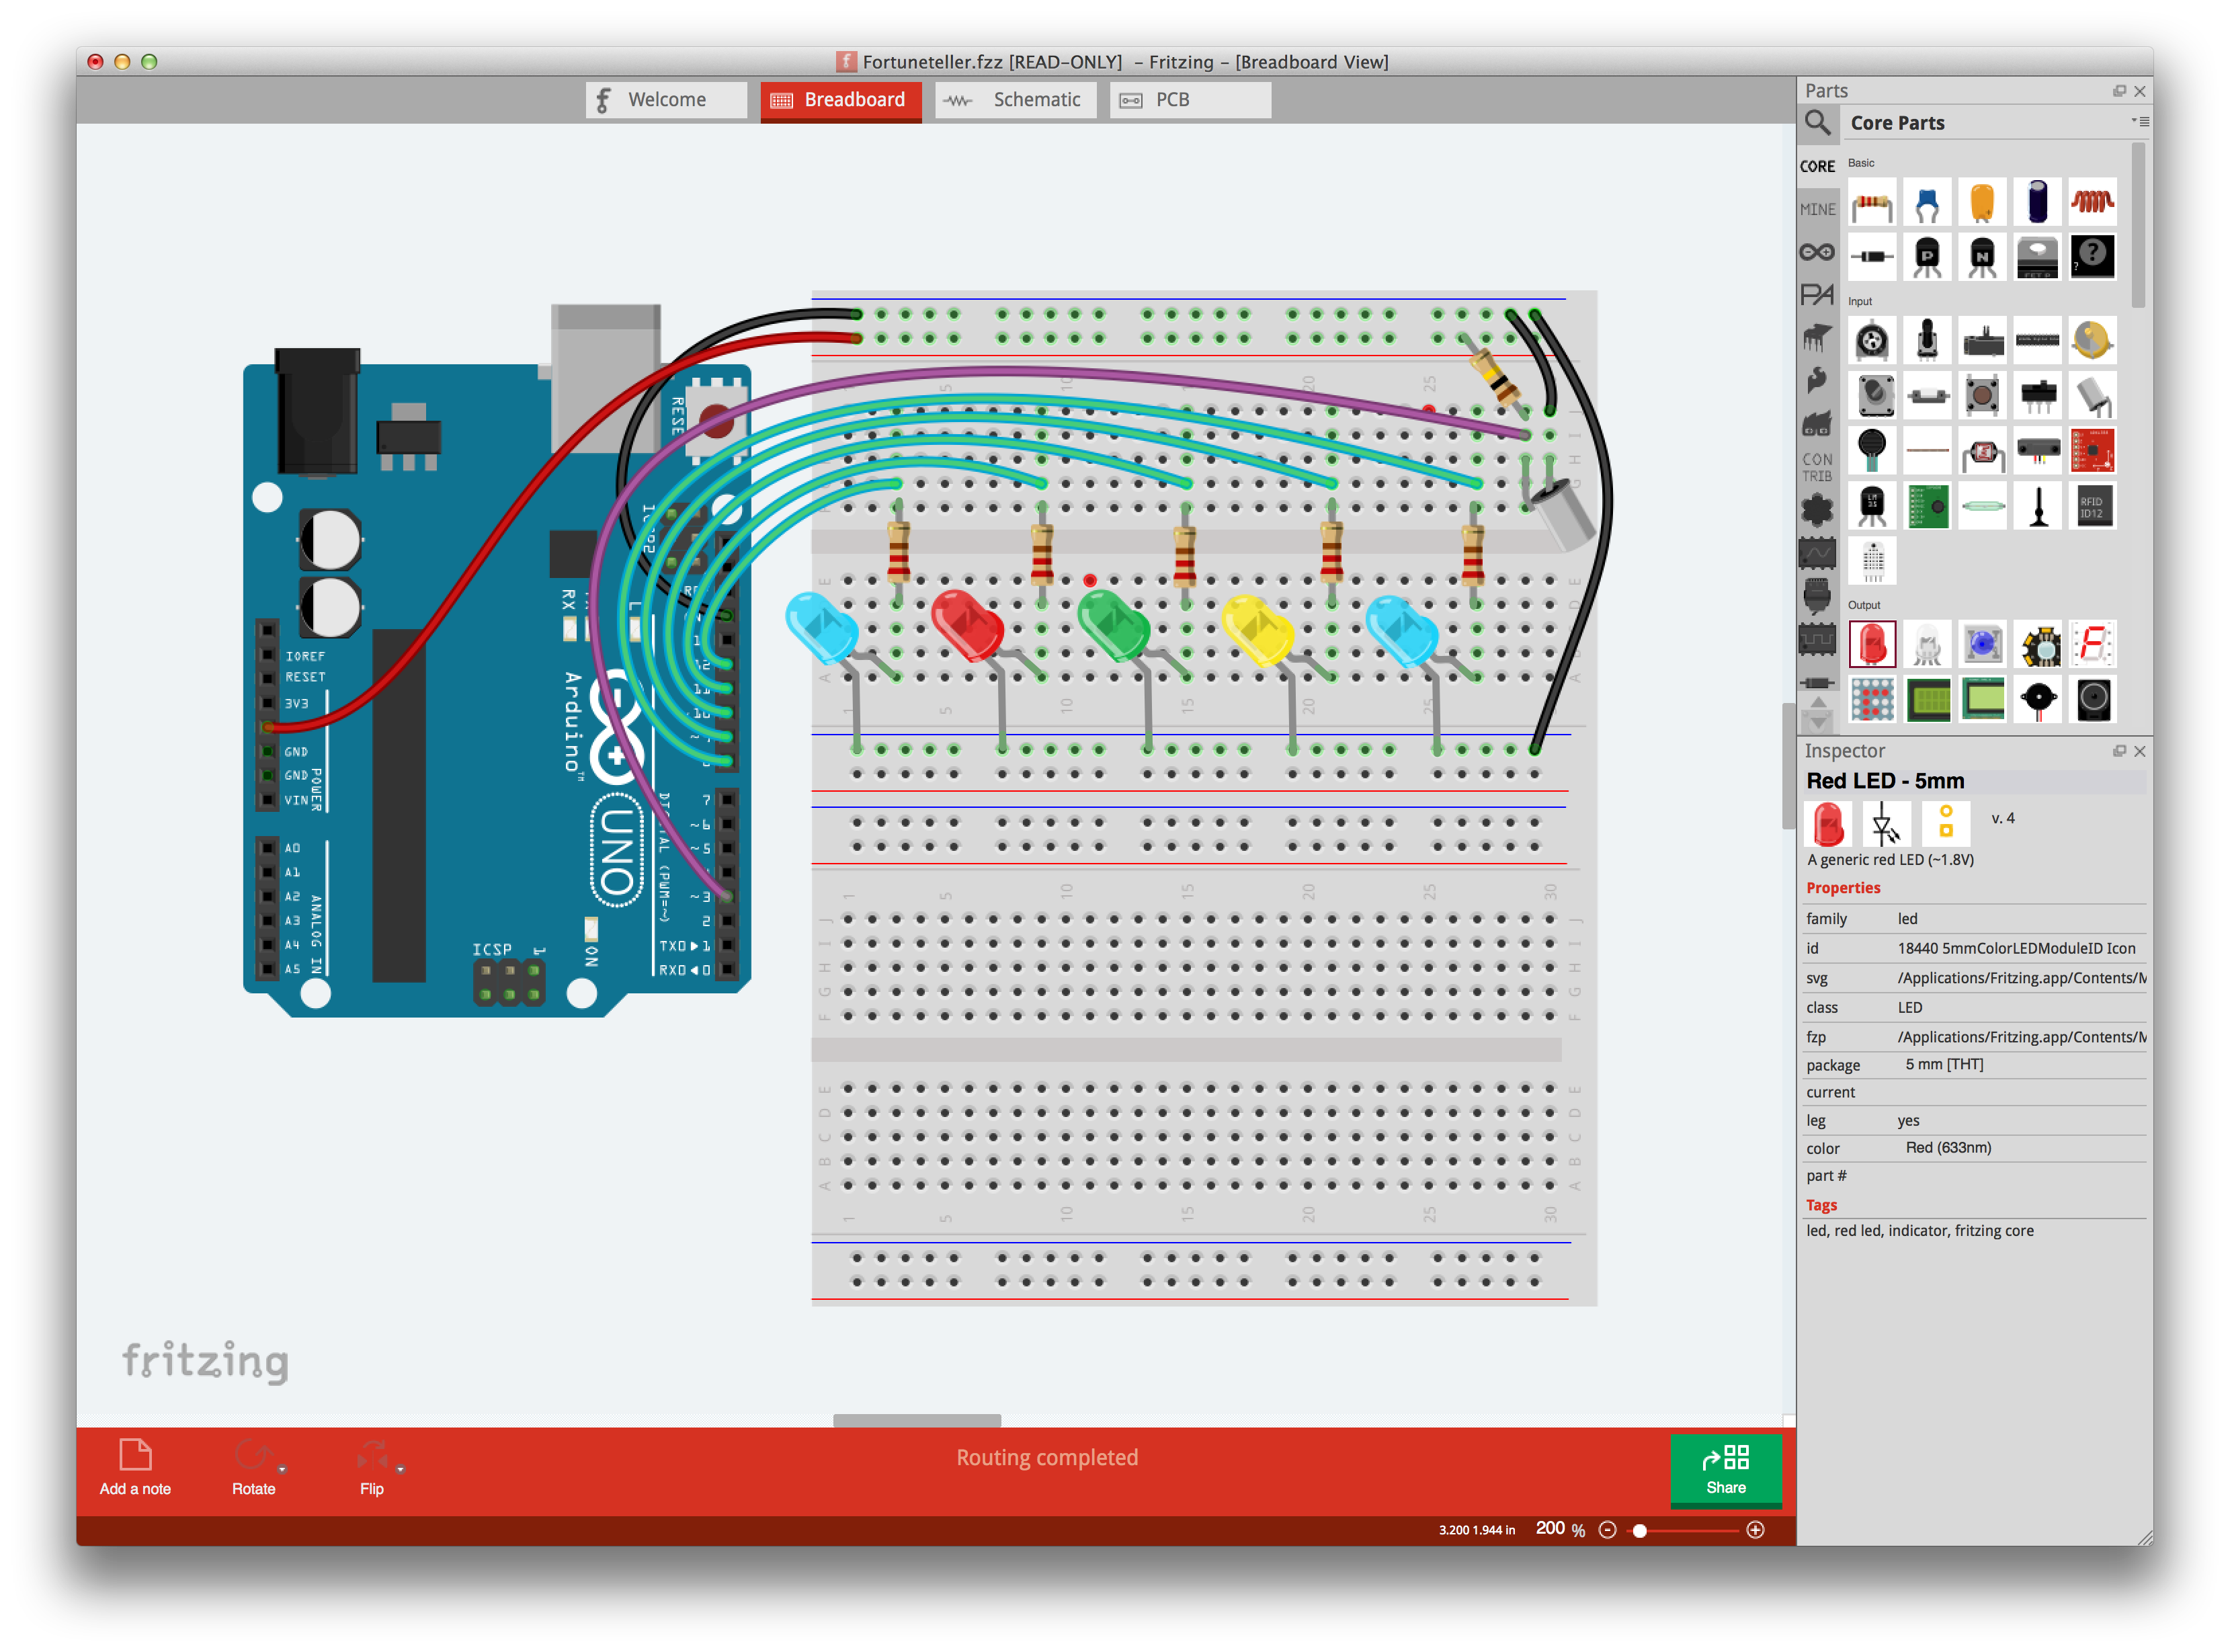
\includegraphics[height=.35\textwidth]{img/FritzingBreadBoard.png}
\caption{Fritizing showing the breadboard environment.}
\label{fig:breadboard}%
\end{figure}


\begin{figure}
\centering
\begin{subfigure}{\columnwidth}
\centering
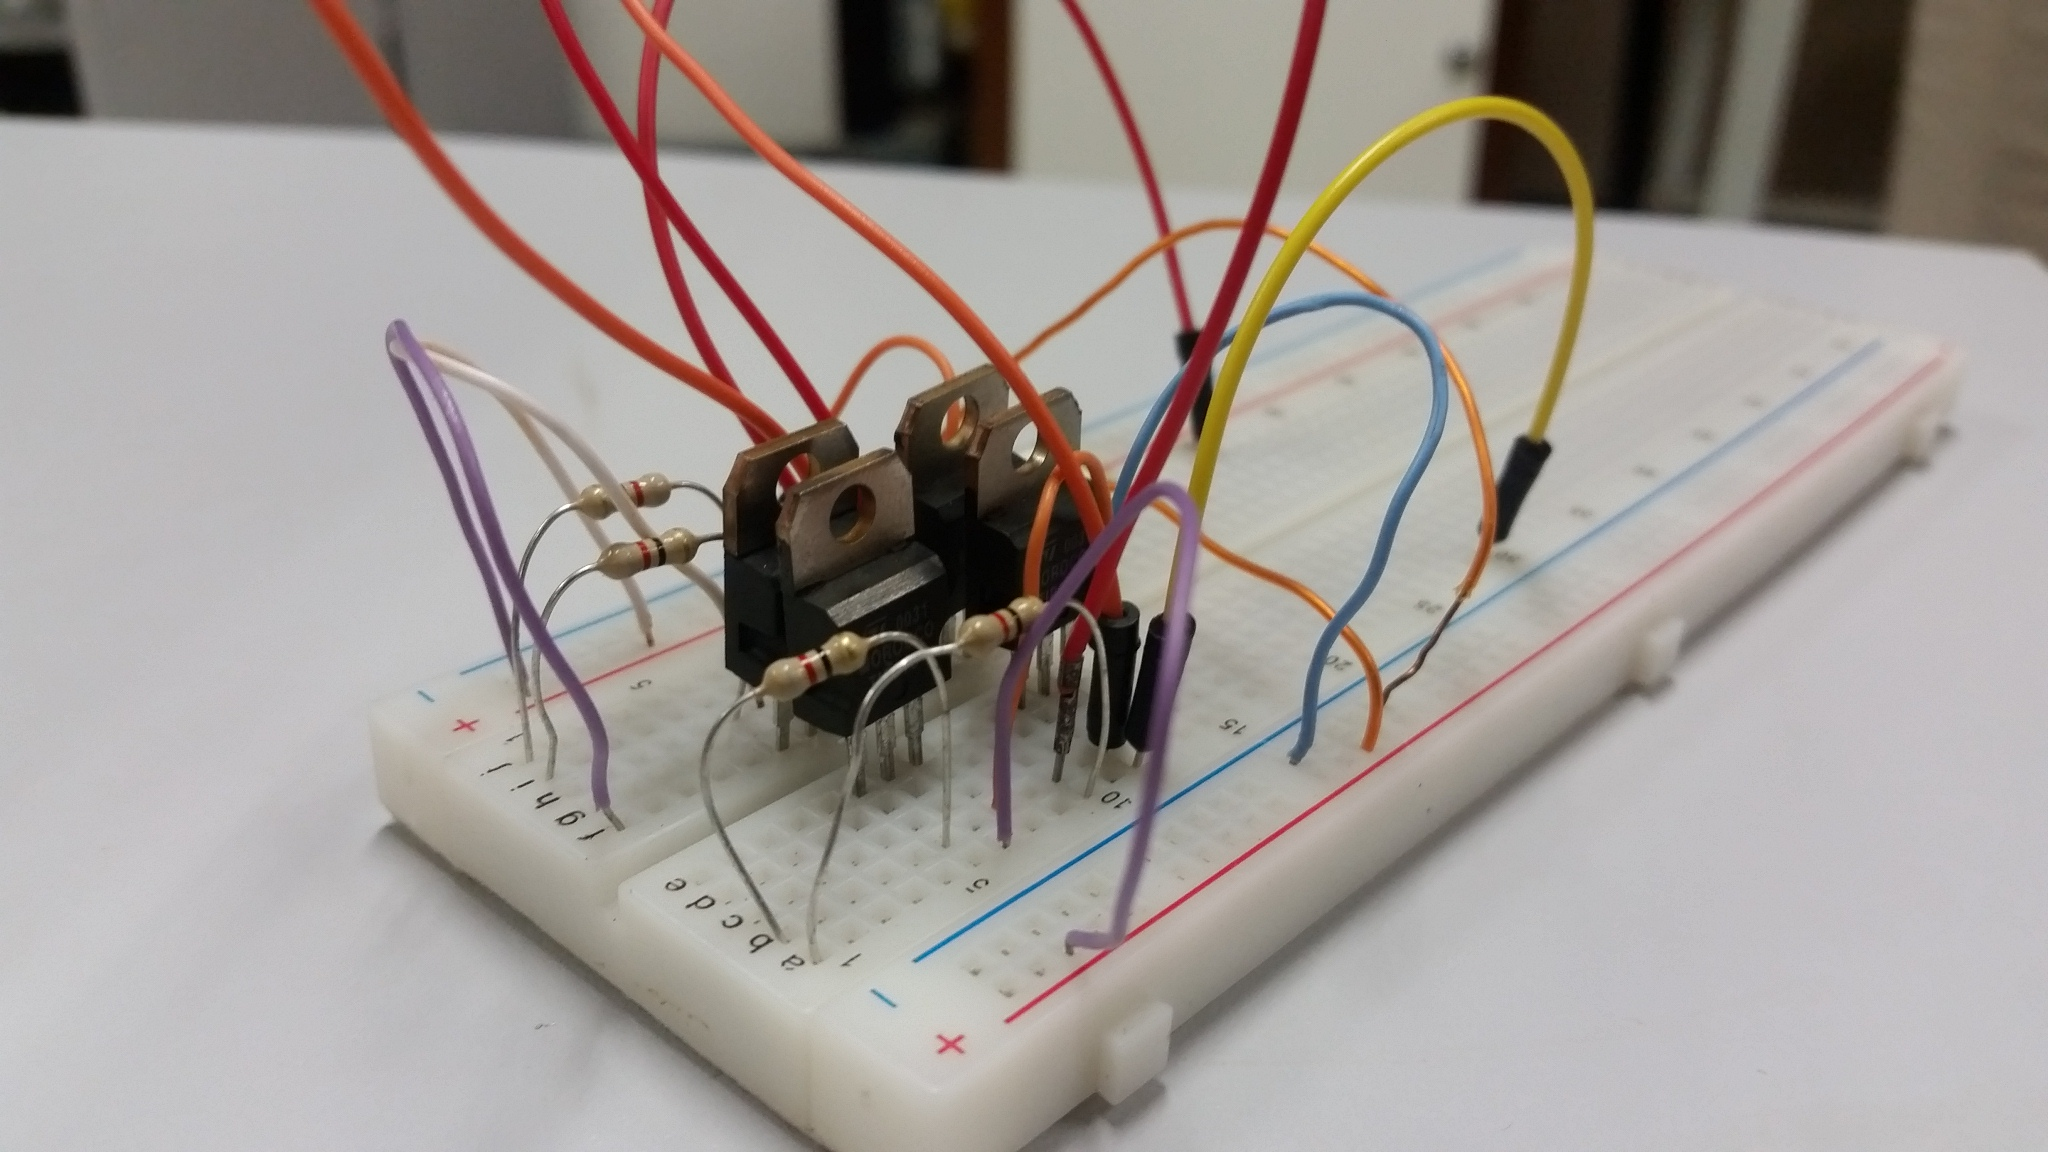
\includegraphics[height=4cm]{img/h_bridge_proto_close.jpg}
\caption{Circuit assembled on a breadboard.}
\label{fig:proto_h}
\end{subfigure}

\begin{subfigure}{.45\columnwidth}
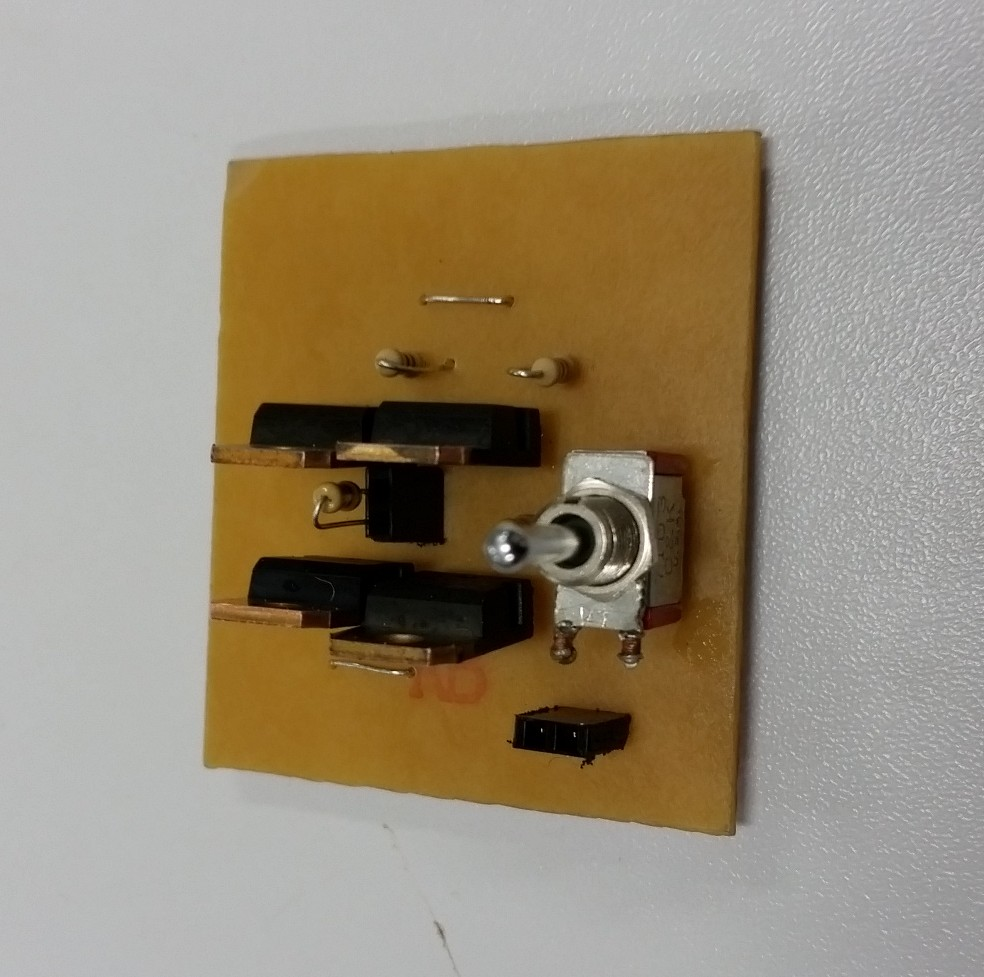
\includegraphics[height=4cm]{img/compontentes4.jpg}
\caption{Components in the PCB.}
\label{fig:pcb_top}
\end{subfigure}
\begin{subfigure}{.45\columnwidth}
\centering
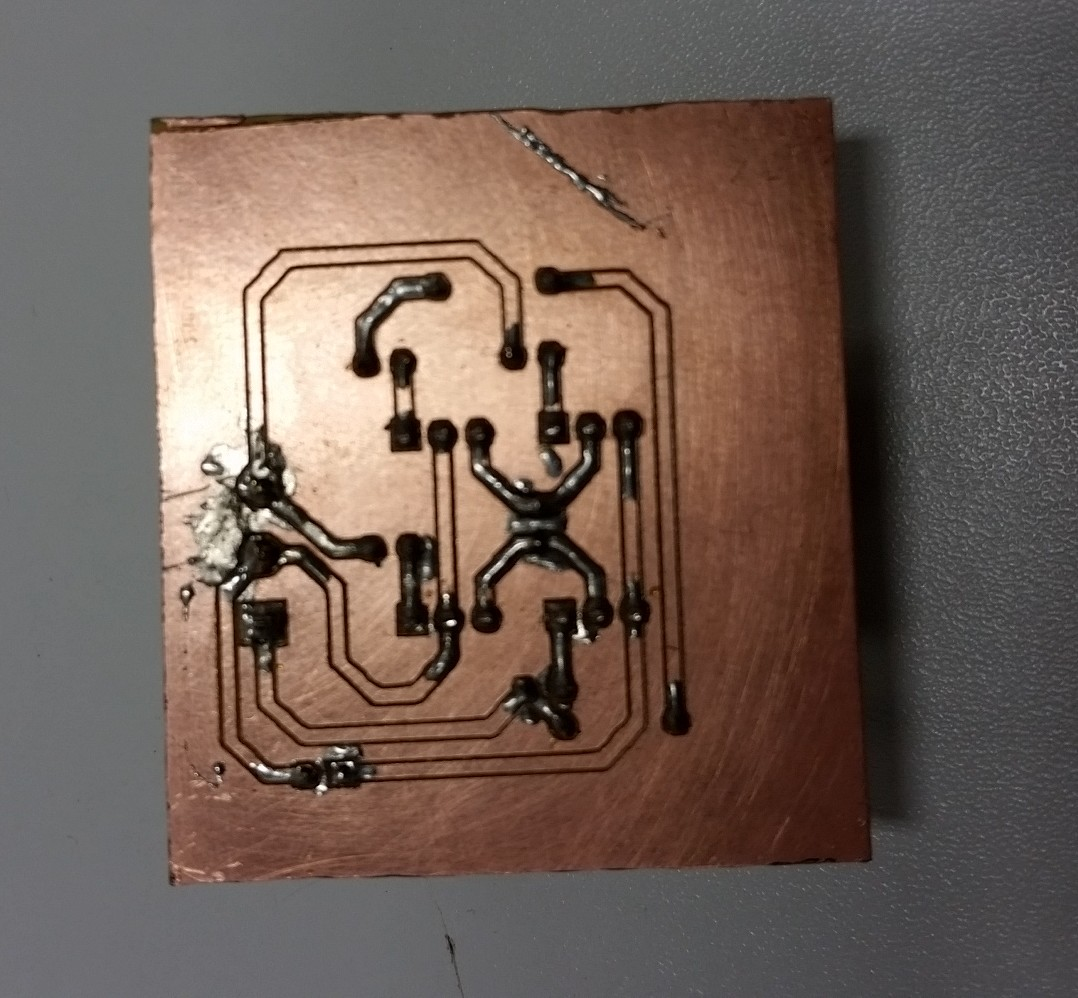
\includegraphics[height=4cm]{img/solda_ja_saiu_da_jaula.jpg}
\caption{Connections in the PCB.}
\label{fig:pcb_bot}
\end{subfigure}

\caption{Circuit assembling.}
\end{figure}
